\begin{frame}[plain]\frametitle{}
\titlepage %表紙
\end{frame}


\begin{frame}\frametitle{紹介論文}
\begin{block}{[Su 15]}
\fullcite{Su2015}
\end{block}
\begin{itemize}
    \item 動画中の人物消去の検出タスク,精度 89\%
    \item K-SVD と K-Means を活用した動画特徴量抽出
    \item クラスタリングを活用した Video Forgery (VF) 関連研究は他にない
\end{itemize}
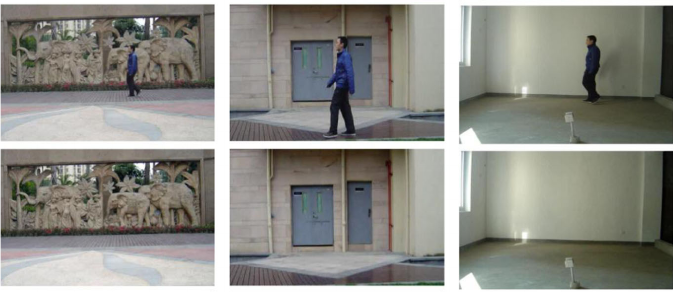
\includegraphics[scale=0.3]{figure/su.png}
\end{frame}


\begin{frame}\frametitle{候補だった論文 1/2}
\begin{block}{[Wang 15]\footfullcite{Wang2015}}
画像の認証・検索で有名な Perceptual Hash 特徴量の改良
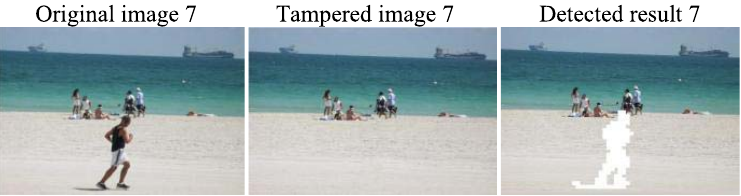
\includegraphics[height=1.5cm]{figure/wang0.png}
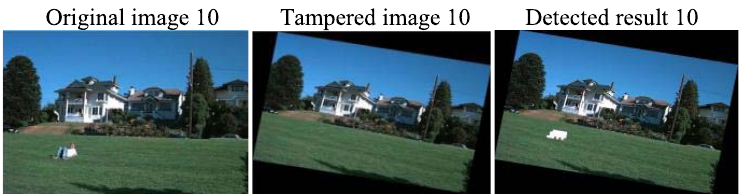
\includegraphics[height=1.5cm]{figure/wang1.png}
\end{block}
下記特徴量を compressive sensing を用いてハッシュ列として統合
\begin{itemize}
    \item Keypoint based feature \\
        変形に頑健な SIFT の Wavelet 低周波成分
    \item Block based feature (改良点) \\
        内容に敏感な Watson's Visual Model (DCT) の低周波成分
\end{itemize}
\end{frame}


\begin{frame}{候補だった論文 2/2}
\begin{block}{[Chen 12]\footfullcite{Chen2012}}
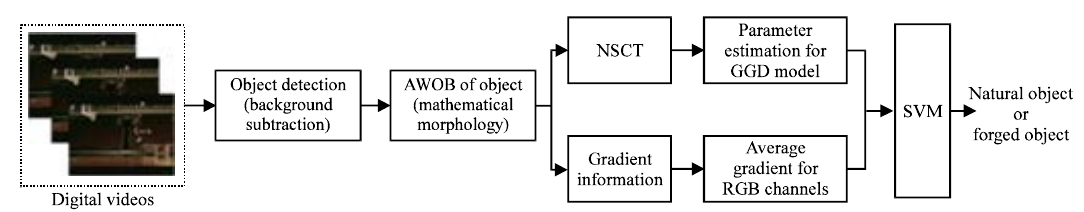
\includegraphics[height=2cm]{figure/chen0.png}
\end{block}

\begin{alertblock}{紹介論文[Su 15] の新規性}
動画データセットからクラスタリングによる統計的な特徴量抽出を行う点が新しい
\end{alertblock}
\end{frame}


% \begin{frame}\frametitle{Overview}
% \begin{alertblock}{[Su 2015] の新規性}
% 訓練データセットから統計的な特徴量抽出を行う点が新しい
% \end{alertblock}
% \begin{block}{論文の構成}
% \begin{enumerate}
%     \item 研究背景や手法の比較
%     \item K-SVD を用いた compressive sensing と形態学的(morphological)な画像処理
%     \item 提案する検出手法
%     \item 実験結果と議論
%     \item まとめ
% \end{enumerate}
% \end{block}
% \end{frame}


\begin{frame}{TOC}
\tableofcontents
\end{frame}
